\subsection{Memory Management in Programming}

Memory management is one of the fundamental challenges in systems and application programming. It determines how memory is allocated, used, and reclaimed during a program's execution. Mismanagement can lead to critical problems such as memory leaks, segmentation faults, or degraded performance. In most programming languages, memory can be divided into two major areas: \textbf{stack memory} and \textbf{heap memory}. These regions serve distinct purposes and are managed in fundamentally different ways. \textbf{Stack memory} is used to store function call frames, including local variables and return addresses. It follows a strict last-in, first-out (LIFO) order, meaning that memory is allocated when a function is called and deallocated automatically when the function returns. This behavior is managed by the compiler and operating system, making stack memory very efficient and deterministic. Importantly, programmers do not need to manually manage stack memory, and issues such as memory leaks or dangling pointers are extremely rare in stack-based memory. \textbf{Heap memory}, on the other hand, is used for dynamic memory allocation when the required lifetime of data is not bound to a function's scope. This memory must be manually allocated and deallocated using functions like \texttt{malloc()} and \texttt{free()} in C/C++. Failure to do so properly can lead to memory safety issues.

To simplify heap memory management and reduce such risks, many modern languages (e.g., Java, Go, Python) incorporate \textbf{garbage collection}, a form of automatic memory management that reclaims unused memory at runtime.

\begin{figure}[h]
\centering
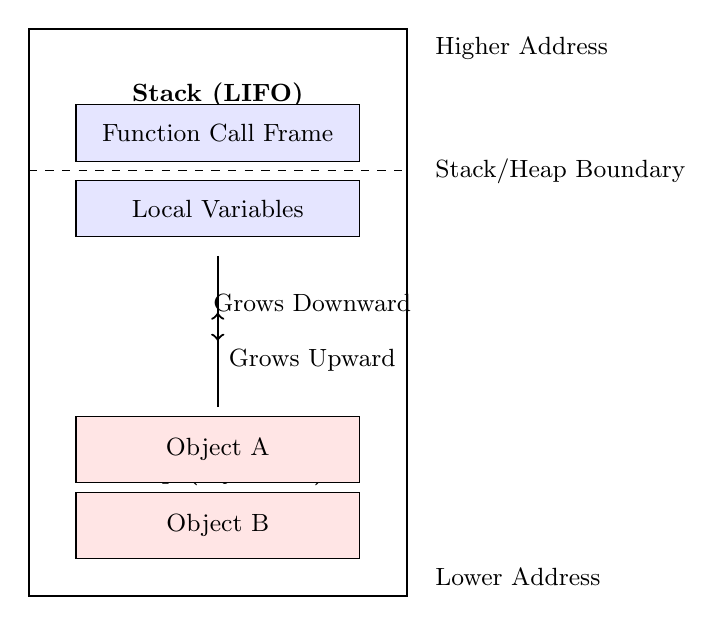
\begin{tikzpicture}[scale=1.2, every node/.style={font=\small}]
% Memory layout
\draw[thick] (0,0) rectangle (4,6);
\node[anchor=west] at (4.2,5.8) {Higher Address};
\node[anchor=west] at (4.2,0.2) {Lower Address};
% Stack region
\draw[dashed] (0,4.5) -- (4,4.5);
\node at (2,5.3) {\textbf{Stack (LIFO)}};
\draw[fill=blue!10] (0.5,4.6) rectangle (3.5,5.2);
\node at (2,4.9) {Function Call Frame};
\draw[fill=blue!10] (0.5,3.8) rectangle (3.5,4.4);
\node at (2,4.1) {Local Variables};
\draw[->, thick] (2,3.6) -- (2,2.7);
\node at (3,3.1) {Grows Downward};

% Heap region
\node at (2,1.3) {\textbf{Heap (Dynamic)}};
\draw[fill=red!10] (0.5,1.2) rectangle (3.5,1.9);
\node at (2,1.55) {Object A};
\draw[fill=red!10] (0.5,0.4) rectangle (3.5,1.1);
\node at (2,0.75) {Object B};
\draw[->, thick] (2,2.0) -- (2,3.0);
\node at (3,2.5) {Grows Upward};

% Label
\node[anchor=west] at (4.2,4.5) {Stack/Heap Boundary};
\end{tikzpicture}
\caption{Stack and Heap Memory Layout in a Typical Program }
\end{figure}

Understanding the differences between stack and heap memory is crucial for analyzing how programming languages manage memory. In the following sections, we will explore how heap memory is managed through manual techniques and automatic algorithms such as garbage collection.

\subsection{Research Motivation and Objectives}

Modern programming languages diverge significantly in their approach to memory management. While languages like C and Rust require manual memory management, offering fine-grained control at the cost of greater developer responsibility, languages like Java, Go, and Python implement automatic memory management through garbage collection. This fundamental difference raises important questions about the performance trade-offs between these approaches. This research aims to systematically investigate how garbage collection impacts application performance in real-world scenarios. While it is commonly accepted that automatic memory management introduces some overhead, the precise nature, extent, and practical implications of this overhead remain insufficiently documented across different types of applications and workloads. The primary objectives of this research are:

\begin{itemize}
    \item To quantify the performance differences between garbage-collected and manually managed languages in both compute-intensive and I/O-intensive tasks 
    \item To identify specific scenarios where garbage collection overhead is most significant 
    \item To analyze how modern garbage collection algorithms perform under different workload patterns 
    \item To provide evidence-based insights for developers making language selection decisions for performance-critical applications 
\end{itemize}

While previous studies have examined language performance differences, they often conflate multiple factors such as runtime environments, compiler optimizations, and language features. This research specifically isolates the impact of garbage collection by controlling for other variables and implementing algorithmically identical solutions across languages.
